\documentclass[a4paper,11pt]{article}
\usepackage[top = 2.5cm, bottom = 2.5cm, left = 2.5cm, right = 2.5cm]{geometry} 
\usepackage[spanish]{babel} %Castellanización
\usepackage[T1]{fontenc}
\usepackage[utf8]{inputenc}
\usepackage{amssymb, amsmath}
\usepackage{multirow}
\usepackage{booktabs}
\usepackage{graphicx}
\usepackage{setspace}
\setlength{\parindent}{0.25in}
\usepackage{float}
\usepackage{fancyhdr}
\usepackage[usenames]{color}
%\documentclass[tikz, border=2mm]{standalone}
\usepackage{karnaugh-map}
\usepackage{graphicx,caption}
\usepackage{verbatim}
\usepackage{hyperref}
\usepackage{algorithmic}
\usepackage{algorithm}
\pagestyle{fancy}
\fancyhf{}

\lhead{\footnotesize INF221: Informe Tarea 2}%
\rhead{\footnotesize CA CS JS - P200}
\cfoot{\footnotesize \thepage} 

\begin{document}


%%%%%%%%%%%%%%%%%%%%%%%%%%%%%%%%%%%%%%%%%%%%%%%%
%%%%%%%%%%%%%%%%%%%%%%%%%%%%%%%%%%%%%%%%%%%%%%%%

\thispagestyle{empty} % This command disables the header on the first page. 

  \begin{minipage}{.2\linewidth}
    \begin{flushleft}
      
\includegraphics[height = 1.5cm]{Imagenes/UTFSM.jpg}
    \end{flushleft}
  \end{minipage}
  \hfill
  \begin{minipage}{.7\linewidth}
    \begin{flushright}
        Universidad Técnica Federico Santa María \\
        Departamento de Informática\\
        INF221 - Algoritmos y Complejidad\\
    \end{flushright}
  \end{minipage}
%\begin{center}
%    \hrule
%\end{center}

\vfill % Now we want to add some vertical space in between the line and our title.
\begin{center}
	{\Large Informe Tarea 2\\}
	{\huge Comparación de Algoritmos de Multiplicación de Matrices\\}
	\vspace{.5cm}
	\hrule
	\vspace{.5cm}
        % YOUR NAMES GO HERE
    {\large Constanza Alvarado V.} - constanza.alvaradov@usm.cl - Rol 201973521-7\\
    {\large Catalina Sierra H.} - catalina.sierrah@usm.cl - Rol 201973557-8\\
	{\large José Southerland S.} - jose.southerland@usm.cl - Rol 201973526-8\\
	
\end{center}
\vfill
\newpage
\section{Introducción}
En el presente informe se realizará una comparación del Algoritmo de Strassen y el Algoritmo Clásico de resolución de Matrices, con la finalidad de poder analizar sus tiempos de ejecución experimentando con distintos valores de $n$ y comparándolos con sus valores téoricos $\Theta(n^{2,81})$ y $\Theta(n^3)$ respectivamente.
\section{Desarrollo}
Para realizar las comparaciones, se crearon dos archivos en lenguaje Python: \texttt{strassen.py} y \texttt{tradicional.py}, que tienen implementados los algoritmos de Strassen y el Clásico respectivamente. Además, se crearon 10 archivos \texttt{.txt} que contienen distintas matrices de tamaño $n\times n$ con valores entre 0 y 9. Los archivos \texttt{.py} piden como input el número del caso que se desea probar; los resultados son mostrados por pantalla junto con el tiempo de ejecución que al programa le tomó calcular la multiplicación.

\section{Resultados}

A continuación se muestran los tiempos de ejecución obtenidos:
\begin{table}[h]
\centering
\begin{tabular}{|l|l|l|}
\hline
\textbf{Matriz $n$} & \textbf{Tradicional [s]} & \textbf{Strassen [s]} \\ \hline
2                         & 0,000032             & 0,00025           \\ \hline
8                         & 0,00018              & 0,00010           \\ \hline
15                        & 0,0026               & 0,00020           \\ \hline
30                        & 0,021                & 0,011             \\ \hline
50                        & 0,036                & 0,025             \\ \hline
100                       & 0,17                 & 0,081             \\ \hline
200                       & 1,19                 & 0,41              \\ \hline
500                       & 19,78                & 1,29              \\ \hline
1000                      & 170,14               & 10,54             \\ \hline
\end{tabular}
\end{table}

Lo cual es representado mediante el siguiente gráfico:
\begin{figure}[h]
    \centering
    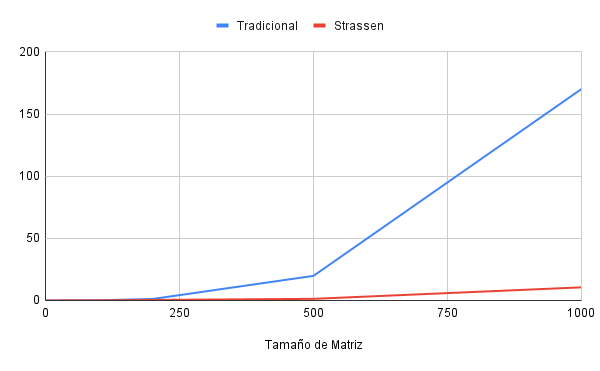
\includegraphics[width=12cm]{Imagenes/graph1.png}
    \caption{Gráfico de resultados de ambos algoritmos.}
    \label{fig:graph1}
\end{figure}
\newpage
Lo cual, traspasado a líneas de tendencia exponenciales se denota así:
\begin{figure}[h]
    \centering
    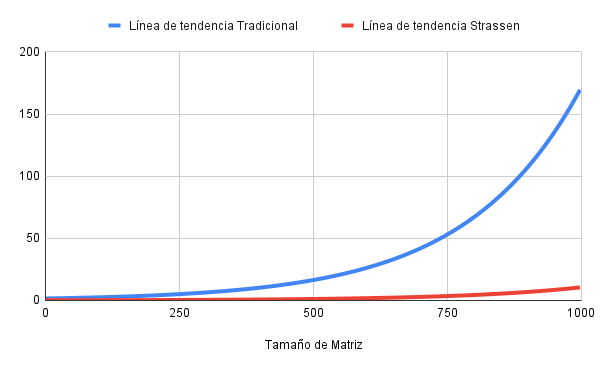
\includegraphics[width=12cm]{Imagenes/graph2.png}
    \caption{Líneas de tendencia de resultados de ambos algoritmos.}
    \label{fig:graph2}
\end{figure}

\section{Conclusión}
A través de los casos probados en ambos algoritmos, se puede concluir que el tiempo de ejecución de ambos algoritmos es exponencial. Sin embargo, el Algoritmo de Strassen tiene una tendencia exponencial menor que el Algoritmo Clásico. Se puede dar cuenta de esto más fácilmente en la diferencia entre el Tiempo de Ejecución para los casos en donde $n$ era 1000. En dicho caso el Algoritmo Clásico dispara su tiempo de ejecución, mientras que en el Algoritmo de Strassen el tiempo aumenta, pero en menor medida.\\

Por lo tanto, se cumple lo mostrado teóricamente: el tiempo de Strassen $\Theta(n^{2,81})$ es exponencial, pero menor que el tiempo del Algoritmo Clásico ($\Theta(n^3)$).
\vfill
\vspace{.5cm}
\hrule
\vspace{.5cm}
\begin{thebibliography}{X}
\bibitem{Libro} \textsc{Arroyuelo D.} Algoritmos Discretos: Análisis y Diseño, Capítulo 11.
\bibitem{Geek} \textsc{Geeks for Geeks} Divide and Conquer: Strassen's Matrix Multiplication. \url{https://www.geeksforgeeks.org/strassens-matrix-multiplication/}
\end{thebibliography}

\end{document}